\documentclass{article}
\usepackage[utf8]{inputenc}
\usepackage{enumerate}
\usepackage{amsmath}
\usepackage{amssymb}
\usepackage{upgreek}
\usepackage{graphicx}
\usepackage{float}
\usepackage{verbatim}
\usepackage{tikz}
\usepackage{cases}
% Zahlenmengen:
\usepackage{dsfont}
%graphen
\usepackage{tikz}
\usepackage{tikzit}
\input{RB_Tree.tikzstyles}

\title{Algo Dat Blatt 07}
\author{Name 1, Name 2,...}
\date{\today}

\begin{document}

\maketitle
\subsection*{Aufgabe 1}
\subsubsection*{Mit TikZit (Grafisches Programm zur tikz Bearbeitung):}
\tikzfig{Tree_01}
\subsubsection*{Direkt als Tikz-Code:}
\usetikzlibrary{trees,automata,positioning}
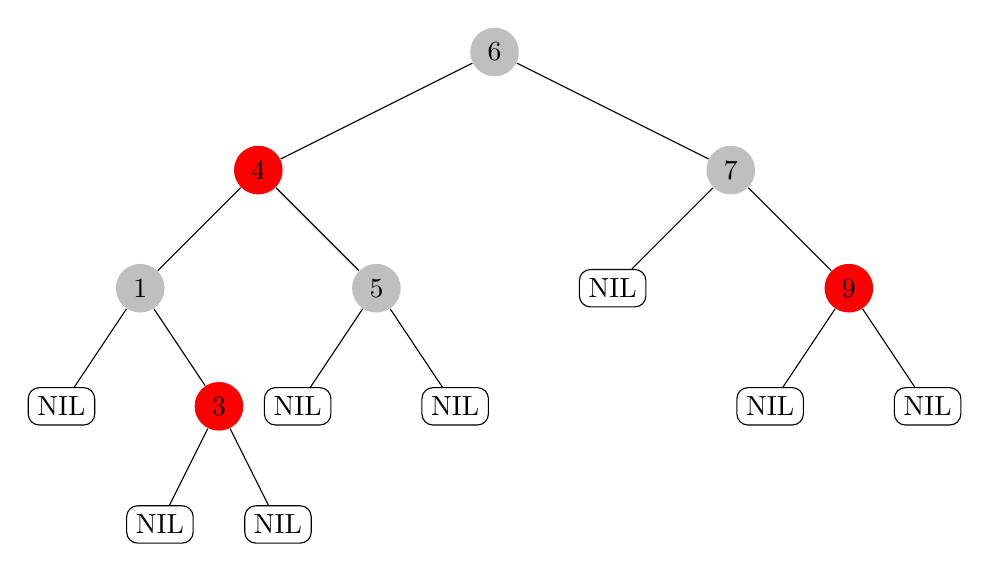
\begin{tikzpicture}[level/.style={sibling distance=60mm/#1}]
\node[circle,fill=lightgray]{$6$}
child {node[circle,fill=red]{$4$}
    child {node[circle,fill=lightgray]{$1$}
        child {node[draw,rounded corners]{NIL}}
        child {node[circle,fill=red]{$3$}
            child {node[rounded corners,draw]{NIL}}
            child {node[rounded corners,draw]{NIL}}}}
    child {node[circle,fill=lightgray]{$5$}
        child {node[rounded corners,draw]{NIL}}
        child {node[rounded corners,draw]{NIL}}}
}
child {node[circle,fill=lightgray]{$7$}
    child {node[rounded corners,draw]{NIL}}
    child{node[circle,fill=red]{$9$}
        child {node[rounded corners,draw]{NIL}}
        child {node[rounded corners,draw]{NIL}}}
};

\end{tikzpicture}
\end{document} 
